\documentclass{article}

\usepackage{lipsum}
\usepackage[margin=1.5in]{geometry}
\usepackage{titlesec}
\usepackage{graphicx}
\usepackage{amsmath}

\usepackage{mathtools, amssymb, nccmath}
\usepackage{bigstrut, changepage, lipsum}

\newcommand{\code}{\texttt}
\newcommand{\norm}[1]{\left\lVert#1\right\rVert}

\usepackage{siunitx} % Required for alignment


% Specify images directory
\graphicspath{ {./report-images/} }

% Header and Footer stuff
\usepackage{fancyhdr}
\pagestyle{fancy}
\fancyhead{}
\fancyfoot{}
\fancyfoot[R]{ \thepage\ }
\renewcommand{\headrulewidth}{0pt}
\renewcommand{\footrulewidth}{0pt}
\newcommand{\sectionbreak}{\clearpage}
\setlength{\parindent}{0pt}

%

\begin{document}

%----------------------------------------------------------------------------------------
%	TITLE PAGE
%----------------------------------------------------------------------------------------

\begin{titlepage} % Suppresses displaying the page number on the title page and the subsequent page counts as page 1
	\newcommand{\HRule}{\rule{\linewidth}{0.5mm}}% Defines a new command for horizontal lines, change thickness here
	
	\center % Centre everything on the page
	
	%------------------------------------------------
	%	Headings
	%------------------------------------------------
	
	\textsc{\Large Data Smoothing}\\[0.5cm] % Major heading such as course name
	
	\textsc{\large Exercise 3}\\[0.5cm] % Minor heading such as course title
	
	%------------------------------------------------
	%	Title
	%------------------------------------------------
	
	\HRule\\[0.6cm]
	
	{\huge\bfseries Data Smoothing Report}\\[0.25cm] % Title of your document
	
	\HRule\\[1.5cm]
	
	%------------------------------------------------
	%	Author(s)
	%------------------------------------------------
	
	\begin{minipage}{0.4\textwidth}
		\begin{flushleft}
			\large
			\textit{Author}\\
			\textsc{Cesare De Cal} % Your name
		\end{flushleft}
	\end{minipage}
	~
	\begin{minipage}{0.4\textwidth}
		\begin{flushright}
			\large
			\textit{Professor}\\
			\textsc{Annie Cuyt}\\ % Supervisor's name
			[0.25cm]
			\textit{Assistant Professor}\\
			\textsc{Ferre Knaepkens} % Supervisor's name

		\end{flushright}
	\end{minipage}
		
	\vfill\vfill\vfill
	
	{\large\today}
		
	\vfill
	
\end{titlepage}

%----------------------------------------------- Introduction ------------------------------------------------------
\section{Introduction}\label{sec:intro}
This exercise asks to use the linearly independent basis function:
$$\phi_{3,i}(x)=\binom{3}{i}x^{i}(1-x)^{3-i}\quad\quad i = 0, 1, 2, 3$$
to find the optimal combination
$$\phi(x)=\lambda_0\phi_{3,0}(x)+\lambda_1\phi_{3,1}(x)+\lambda_2\phi_{3,2}(x)+\lambda_3\phi_{3,3}(x)$$
that minimizes the Euclidean norm
$$\sqrt{\sum_{j=0}^{19}{(\phi(x_j)-y_j)^2}}$$
for the 20 data points $(x_j,y_j)$ given in

\begin{table}[!ht]
\large        %% not "\fontsize{12}{12}\selectfont"
\centering    %% not "\center{...}"
\begin{tabular}{|c|c|c|}
\hline
$j$ & $x_j$ & $y_j$ \\     %% no "&" at start of row
\hline
0 & 0.0 & -0.80\\
1 & 0.6 & -0.34\\
2 & 1.5 & 0.59\\
3 & 1.7 & 0.59\\
4 & 1.9 & 0.23\\
5 & 2.1 & 0.10\\
6 & 2.3 & 0.28\\
7 & 2.6 & 1.03\\
8 & 2.8 & 1.50\\
9 & 3.0 & 1.44\\
10 & 3.6 & 0.74\\
11 & 4.7 & -0.82\\
12 & 5.2 & -1.27\\
13 & 5.7 & -0.92\\
14 & 5.8 & -0.92\\
15 & 6.0 & -1.04\\
16 & 6.4 & -0.79\\
17 & 6.9 & -0.06\\
18 & 7.6 & 1.00\\
19 & 8.0 & 0.00\\    
\hline
\end{tabular}
\end{table}

This is an overdetermined system. To solve this exercise, I'll first find the coefficient matrix $A$ and then use $QR$ decomposition to solve the system. I'll also calculate the $l_2$-norm of the residual, and the condition number of the coefficient matrix. Finally, I'll plot the data points with the graph of the function $\phi(x)$.

%---------------------------------- Introduction ------------------------------------------------------
\section{Tools}
The following programming language and libraries have been used in this exercise:
\begin{itemize}
  \item C
  \item GSL (GNU Scientific Library)
  \item C Math Library
  \item Python (for plotting)
  \item SciPy (for plotting)
\end{itemize}
The following double-precision GSL data types have been used in the exercise:
\begin{itemize}
  \item \code{gsl\_matrix}
  \item \code{gsl\_vector}
\end{itemize}
The following GSL methods have been used in the exercise:
\begin{itemize}
  \item \code{gsl\_matrix\_alloc(size1, size2)}
  \item \code{gsl\_matrix\_set(matrix, row, column, value)}
  \item \code{gsl\_matrix\_get(matrix, row, column)}
  \item \code{gsl\_vector\_alloc(size)}
  \item \code{gsl\_vector\_set(vector, index, value)}
  \item \code{gsl\_vector\_set\_zero(vector)}
  \item \code{gsl\_vector\_get(vector, index)}
  \item \code{gsl\_matrix\_memcpy(destinationMatrix, matrixToCopyFrom)}
  \item \code{gsl\_linalg\_SV\_decomp(A, V, S, workspaceVector)}
  \item \code{gsl\_vector\_minmax(vector, minInVector, maxInVector)}
  \item \code{gsl\_sf\_fact(number)} to calculate the factorial
  \item \code{gsl\_sf\_pow\_int(base, exponent)}
  \item \code{gsl\_blas\_dnrm2(vector)} to calculate the Euclidean norm
  \item \code{gsl\_matrix\_free(matrixToDeallocate)}
  \item \code{gsl\_vector\_free(vectorToDeallocate)}
\end{itemize}
In order to decompose the coefficient matrix into its QR decomposition, and then solve the square system $A\vec{x}=\vec{b}$, I've used the following methods:
\begin{itemize}
  \item \code{gsl\_linalg\_QR\_decomp(matrixQR, vectorTau)}
  \item \code{gsl\_linalg\_QR\_lssolve(matrixQR, vectorTau, vectorB, vectorX, vectorResidual)}
  \item \code{gsl\_permutation\_alloc(size)}
\end{itemize}
The following method from the C Math library was used in this exercise to calculate the absolute value of a number:
\begin{itemize}
  \item \code{fabs(x)}
\end{itemize}
  
\section{Computation}
First of all, I compute the coefficients A of the linear system by using the linearly independent basis function. For the $(i, j)$ cell in the matrix, I call the basis function by passing the $i$-th element of the $x$ data points, and by using the column $j$ for the $i$ parameter of the basis function. This results in a $20\times4$ matrix. The following is a representation of A:
\begin{adjustwidth}{-2em}{-2em}
    \[ \medmath{\begin{bmatrix*}[r]
1.000000000000000\,e+00 & 0.000000000000000\,e+00 & 0.000000000000000\,e+00 & 0.000000000000000\,e+00 \bigstrut[t]\\
6.400000000000002\,e-02 & 2.880000000000000\,e-01 & 4.320000000000001\,e-01 & 2.160000000000000\,e-01 \\
-1.250000000000000\,e-01 & 1.125000000000000\,e+00 & -3.375000000000000\,e+00 & 3.375000000000000\,e+00 \\
-3.429999999999999\,e-01 & 2.499000000000000\,e+00 & -6.068999999999998\,e+00 & 4.912999999999999\,e+00 \\
-7.289999999999998\,e-01 & 4.616999999999998\,e+00 & -9.747000000000000\,e+00 & 6.858999999999999\,e+00 \\
-1.331000000000000\,e+00 & 7.623000000000002\,e+00 & -1.455300000000000\,e+01 & 9.261000000000001\,e+00 \\
-2.196999999999999\,e+00 & 1.166100000000000\,e+01 & -2.063099999999999\,e+01 & 1.216700000000000\,e+01 \\
-4.096000000000001\,e+00 & 1.996800000000001\,e+01 & -3.244800000000000\,e+01 & 1.757600000000000\,e+01 \\
-5.831999999999998\,e+00 & 2.721599999999999\,e+01 & -4.233599999999999\,e+01 & 2.195199999999999\,e+01 \\
-8.000000000000000\,e+00 & 3.600000000000000\,e+01 & -5.400000000000000\,e+01 & 2.700000000000000\,e+01 \\
-1.757600000000000\,e+01 & 7.300800000000001\,e+01 & -1.010880000000000\,e+02 & 4.665600000000001\,e+01 \\
-5.065300000000001\,e+01 & 1.930290000000000\,e+02 & -2.451990000000000\,e+02 & 1.038230000000000\,e+02 \\
-7.408800000000001\,e+01 & 2.751840000000000\,e+02 & -3.407040000000000\,e+02 & 1.406080000000000\,e+02 \\
-1.038230000000000\,e+02 & 3.777390000000001\,e+02 & -4.581090000000000\,e+02 & 1.851930000000000\,e+02 \\
-1.105920000000000\,e+02 & 4.008960000000000\,e+02 & -4.844160000000000\,e+02 & 1.951120000000000\,e+02 \\
-1.250000000000000\,e+02 & 4.500000000000000\,e+02 & -5.400000000000000\,e+02 & 2.160000000000000\,e+02 \\
-1.574640000000000\,e+02 & 5.598720000000002\,e+02 & -6.635520000000001\,e+02 & 2.621440000000001\,e+02 \\
-2.053790000000000\,e+02 & 7.205670000000001\,e+02 & -8.426970000000001\,e+02 & 3.285090000000001\,e+02 \\
-2.874960000000000\,e+02 & 9.931679999999998\,e+02 & -1.143648000000000\,e+03 & 4.389759999999999\,e+02 \\
-3.430000000000000\,e+02 & 1.176000000000000\,e+03 & -1.344000000000000\,e+03 & 5.120000000000000\,e+02 \bigstrut[b]
\end{bmatrix*}} \]%
\end{adjustwidth}

% --------- CONDITION NUMBER ---------
Then, I calculate the condition number of the coefficient matrix $A$. In GSL there is no direct function that calculates the condition number, but it's possible to use the ratio of the largest singular value of matrix A, $\sigma_n (A)$, to the smallest $\sigma_1 (A)$:

$$\kappa(A) := \frac{\sigma_n (A)}{\sigma_1 (A)}= \frac{\norm{A}}{\norm{A^{-1}}^{-1}}$$

I proceed to factorize $A$ into its singular value decomposition $SVD$ using the \code{gsl\_linalg\_SV\_decomp} method, and then use $\code{gsl\_vector\_minmax}$ to extract the minimum and maximum singular values out of the vector $S$ that contains the diagonal elements of the singular value matrix. The condition number of the matrix $A$ is equal to $3.741019262503867e+03$.\\

% --------- CONDITION NUMBER ---------

The column vector $\vec{b}$ is formed by the input $y_j$ values:
$$
\begin{bmatrix} 
-8.000000000000000e-01\\
-3.400000000000000e-01\\
5.900000000000000e-01\\
5.900000000000000e-01\\
2.300000000000000e-01\\
1.000000000000000e-01\\
2.800000000000000e-01\\
1.030000000000000e+00\\
1.500000000000000e+00\\
1.440000000000000e+00\\
7.400000000000000e-01\\
-8.200000000000000e-01\\
-1.270000000000000e+00\\
-9.200000000000000e-01\\
-9.200000000000000e-01\\
-1.040000000000000e+00\\
-7.900000000000000e-01\\
-6.000000000000000e-02\\
1.000000000000000e+00\\
0.000000000000000e+00\\
\end{bmatrix}
$$

I proceed in solving the system (finding the $\lambda$ values that approximate to a solution of the system). I use QR decomposition to solve the system ($\code{gsl\_linalg\_QR\_decomp}$ and $\code{gsl\_linalg\_QR\_lssolve}$ GSL methods). The following is the QR decomposition of A:

\begin{adjustwidth}{-2em}{-2em}
    \[ \medmath{\begin{bmatrix*}[r]
-5.607137694902810e+02 & 1.956202843752372e+03 & -2.276212763756861e+03 & 8.833928944999552e+02 \\
1.139370324819986e-04 & -4.671135706796601e+01 & 1.122030535262658e+02 & -6.782418228480103e+01 \\
-2.225332665664034e-04 & 1.460497799957120e-02 & 7.581872706318327e+00 & -8.735870723873337e+00 \\
-6.106312834582108e-04 & 2.762429988027977e-02 & 1.797466673315370e-01 & -2.470454024049311e+00 \\
-1.297814010615264e-03 & 4.400918925292650e-02 & 2.113118885654055e-01 & 1.354991299702775e-01 \\
-2.369534222399064e-03 & 6.326913656703972e-02 & 2.350053228690535e-01 & 9.686987975376644e-02 \\
-3.911244693171105e-03 & 8.491363227214763e-02 & 2.513310790520081e-01 & 6.050043190845661e-02 \\
-7.291970078847909e-03 & 1.207784144212678e-01 & 2.631080548709738e-01 & 1.049772432830278e-02 \\
-1.038251208492211e-02 & 1.462383018205487e-01 & 2.632200917938682e-01 & -1.959354810540480e-02 \\
-1.424212906024982e-02 & 1.723659541841733e-01 & 2.577288314294048e-01 & -4.692208258102275e-02 \\
-3.128995754536886e-02 & 2.498504055563917e-01 & 2.126763547071380e-01 & -1.108942994397425e-01 \\
-9.017582041110428e-02 & 3.520968788593226e-01 & 5.605686650054093e-02 & -1.473630562460556e-01 \\
-1.318963572269736e-01 & 3.635568863958127e-01 & -2.831753402090372e-02 & -1.240982343374392e-01 \\
-1.848325706777897e-01 & 3.424022086740725e-01 & -1.099043818739413e-01 & -7.278910904340619e-02 \\
-1.968831921288935e-01 & 3.335830602668363e-01 & -1.251940955112117e-01 & -5.896438574071358e-02 \\
-2.225332665664034e-01 & 3.108660410390103e-01 & -1.542417580429807e-01 & -2.760834500928011e-02 \\
-2.803278262928973e-01 & 2.434003295032724e-01 & -2.044456433018340e-01 & 5.043304854412397e-02 \\
-3.656292780331310e-01 & 1.127004233192019e-01 & -2.472054281433762e-01 & 1.782091144383195e-01 \\
-5.118193920381977e-01 & -1.705668773785795e-01 & -2.556299463550832e-01 & 4.175378294298211e-01 \\
-6.106312834582110e-01 & -3.921595584433181e-01 & -2.261060282111244e-01 & 5.880648466528077e-01 \\
\end{bmatrix*}} \]%
\end{adjustwidth}

The solutions vector is directly given by the $\code{gsl\_linalg\_QR\_lssolve}$ method.

$$
\begin{bmatrix}
-1.118262027055321e+00\\
-4.515724133992401e-01\\
2.972563550105292e-03\\
2.972882574075207e-01\\
\end{bmatrix}
$$

The residual vector $\vec{r}$ is also directly given by the $\code{gsl\_linalg\_QR\_lssolve}$ method.
$$
\begin{bmatrix}
3.182620270553753e-01\\
-2.038767862631474e-01\\
-3.507925507654632e-02\\
-1.076211346528342e-01\\
-5.104297656943454e-01\\
-6.559970851745927e-01\\
-4.668150300670836e-01\\
3.379120178166642e-01\\
8.680652851344475e-01\\
8.842461476326978e-01\\
4.840349364751467e-01\\
-4.332442092900336e-01\\
-6.426370573997744e-01\\
-1.387527086448619e-01\\
-1.218089886087358e-01\\
-2.242466352247385e-01\\
-1.314405461740510e-02\\
5.037445845512266e-01\\
8.885672158267567e-01\\
-7.311795037780225e-01\\
\end{bmatrix} 
$$

The Euclidean norm of the residual vector, which can be easily calculated with $\code{gsl\_blas\_dnrm2(vector)}$, is equal to $2.282876480420795e+00$.
\section{Plot}

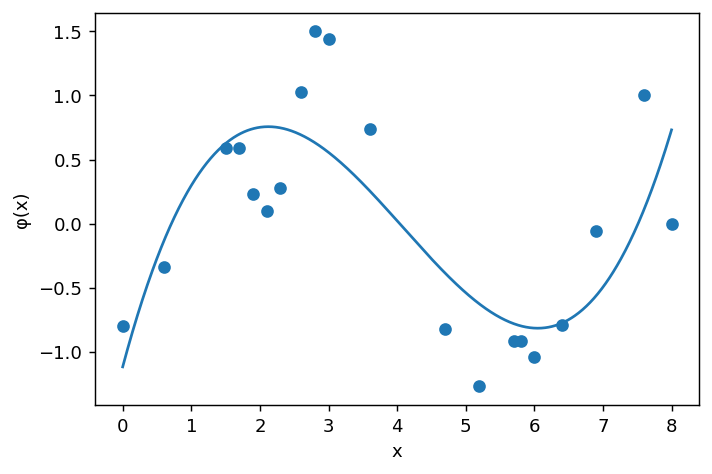
\includegraphics[width=\textwidth,height=\textheight,keepaspectratio]{graph.png}

\section{Observations}
In this problem I have worked with an overdetermined system of equations which has more equations that unknowns ($m >> n \rightarrow20 >> 4$). It is not possible to find the exact $\vec{x}$ vector, but I found a set of $lambda$ that satisfies the system as close as possible through $QR$ factorization. \\

At the end of the exercise, I plotted the computed function together with the data points. In order to plot the graph of the $\phi(x)$ function, I used the $\lambda$ values contained in $\vec{x}$ and plugged them into the linear combination. Plus, I created an array of equidistant $x$ values and calculated the function value for each of the values. We can observe that the function gives a general of the data points, but overall I don't think it is very accurate.

\end{document}